
\section{Problem Formulation} 
 
Given a subset of data and attributes to be studied, the goal for {\tt VizInNuce} is to  identify the most interesting and informative visualizations summarizing patterns or trends. There are two major challenges in achieving this goal; (i) scale: evaluating a large number of candidate visualizations in lattice while responding within interactive time scales, and (ii) utility: identifying appropriate metrics for assessing interestingness and informativeness of visualizations. For now, we focus on the latter. We first describe two conceptual visualization lattices, and then describe the .


\iffalse
\subsection{}

Given a relational dataset, our goal is to identify the most interesting and informative visualizations from the dataset summarizing patterns or trends of interest. We have the following aspects of interest: 
  \begin{itemize}
    \item Visualizations in a dashboard should present a connected story, i.e., there should be connections/relationships among the chosen visualizations.
    \item These connections/relationships should be informative rather than misleading.
    \item We are interested in the informative, yet surprising relationships. Surprisingness arises when the relationships deviate from expected traits.
    \item Each visualization should cover a significant population. Surprising relationships appearing in the low levels of data (e.g., 0.1\% of tuples) are not of interest.
  \end{itemize}
 \fi
 
 
\subsection{Preliminaries} 
A dataset $D$ consists of a set of dimension attributes $A$, and a set of measure attributes $M$. We define a metric family $z$ as the result of a SQL query using a group of dimension attributes $A_z \subseteq A$, a single measure attribute $m_z \in M$, and an aggregate function $f_z$ as follows: {\tt SELECT $A_z$ AS $metric\_id, f(m_z)$ AS $metric\_value$ FROM $D$ GROUP BY $A_z$}. The result of this query can be presented using a table with two columns, where the first column accommodates the metrics within the metric family, and the second column accommodates the values corresponding to these metrics. This two column table can be visualized with a bar chart, where each metric is visualized using a separate bar. 
\newline
\newline
Notice that the aforementioned query does not have a {\tt WHERE} clause. If we include a {\tt WHERE} clause in this query incorporating constraints on the remaining dimension attributes $A_z^\prime = A - A_z$, we shall get different instances of $z$ corresponding to different data subsets defined by the constraints. These different instances of $z$ can be visualized with separate bar charts that present the same metric family for different data subsets. 

\subsection{Data Subset Lattice}
A data subset can be contained within another data subset. Specifically, given a data subset defined by a set of constraints on dimension attributes, adding one or more new constraints in the set will generate a new data subset that is contained within the former subset. We specify a data subset as the \emph{parent} of another data subset if the latter is defined by a set of constraints that includes one additional constraint along with the ones that define the former subset. Notice that, as per our definition, a data subset can have multiple parent subsets.
 \newline
 \newline
We extend the idea of parent data subset to introduce the concept of parent visualization. Let $V_s(z)$ represent the set of visualizations that visualize a metric family $z$ for different data subsets. Given a visualization $v_i \in V_s(z)$ (corresponding to a particular data subset), parent of $v_i$, $v_i^j \in V_s(z)$ is a visualization that corresponds to a parent data subset of the former. Analogous to a data subset, a visualization $v_i \in V_s(z)$ can have multiple parents. 

\begin{figure*}[bht]
\label{example}
\centering
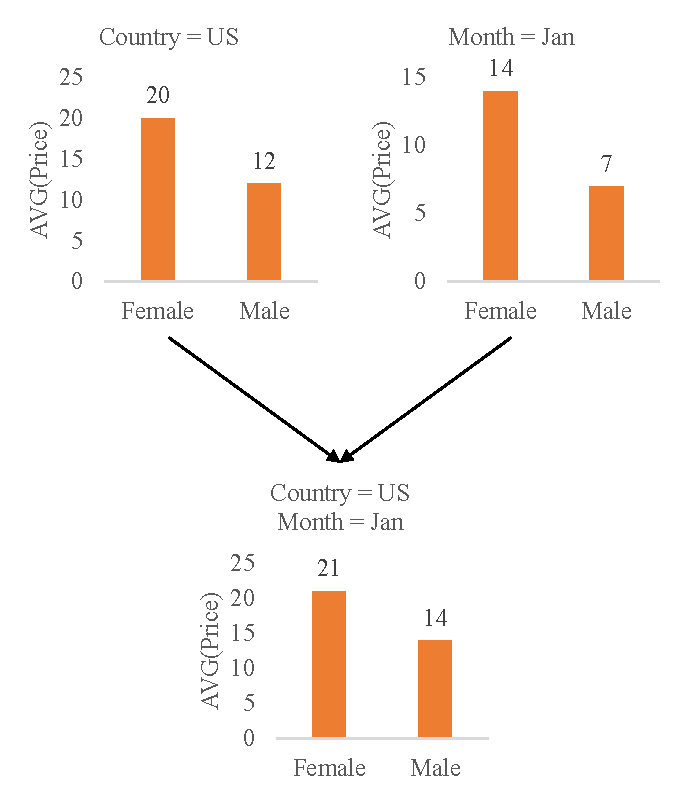
\includegraphics[scale=0.75]{SubsetRelation.pdf}
\caption{Parent Child Relationship in Data Subset Lattice}
\end{figure*}
 



\subsection{Dimension Combination Lattice}
Given a combination of dimension attributes, inducing one or more new dimensions in the combination will generate a new combination. We specify a dimension combination as the \emph{parent} of another dimension combination if the latter is defined by a set of dimensions that includes one additional dimension along with the ones that define the former combination. Notice that, as per our definition, a dimension combination can have multiple parent combinations.
 \newline
 \newline
Let $V_c(Z)$ represent the set of visualizations that visualize the different metric families with same measure of interest and same data subset. We extend the idea of parent dimension combination to introduce the concept of parent visualization. Specifically, given a visualization $v_i \in V_c(Z)$ (corresponding to a particular dimension combination), parent of $v_i$, $v_i^j \in V_c(Z)$ is a visualization that corresponds to a parent dimension combination of the former. Analogous to a dimension combination, a visualization $v_i \in V_c(Z)$ can have multiple parents. 

\begin{figure*}[bht]
\label{example}
\centering
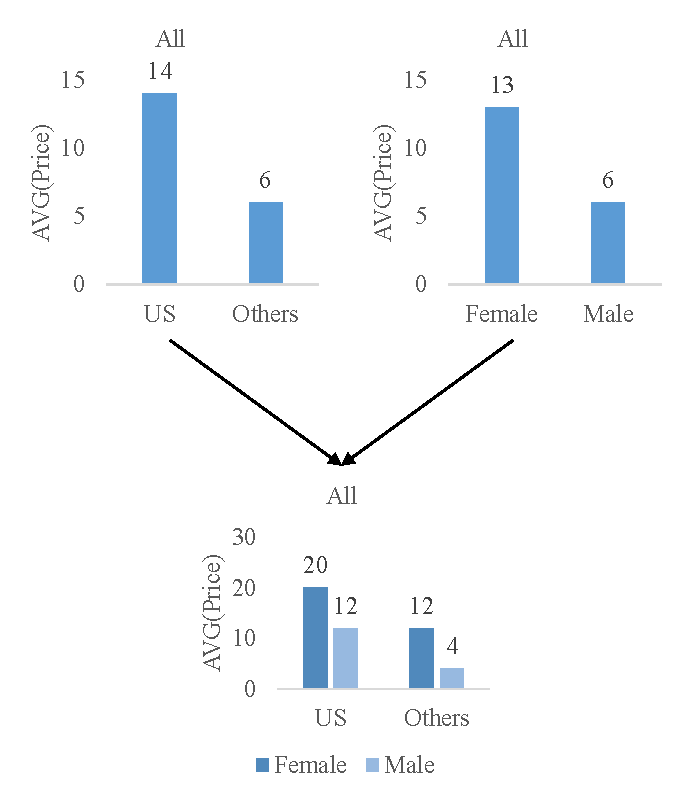
\includegraphics[scale=0.75]{DimensionRelation.pdf}
\caption{Parent Child Relationship in Dimension Combination Lattice}
\end{figure*}
 


\section{Parent Child Relationship Model} 
We observe that, while exploring a dataset, users first look at the top level visualizations before looking at the next level. Further, the knowledge learnt from the top level visualizations set up user expectation for the next level. Based on these two observations, we quantify the parent-child relationship mentioned above.  
  
\subsection{User Expectation Model}
We formulate user expectation ($\hat{v_i}$) corresponding to a visualization $v_i$, based on its parents, $v_i^1, \ldots, v_i^\lambda$. 
  
$$\hat{v_i} = g(v_i^1, \ldots, v_i^\lambda)$$

Here, the function $g()$ takes the parents of $v_i$ as argument and returns user expectation $\hat{v_i}$.
\newline
\newline
We assert that the parents of $v_i$ do not contribute equally in setting up user expectation $\hat{v_i}$. We care about the $p$ parents that contribute most in setting up $\hat{v_i}$. We call these $p$ parents the \emph{true parents} of $v_i$ and represent them as $[v_i^*, p]$. 
  
$$[v_i^*,p] = \underset{v_i^j}{\operatorname{arg\,\,\,max\_p}}\ d(v_i,v_i^j)$$
  %better expressed as top_p_v_i^j??
Here, the function $d()$ takes $v_i$ and its parent $v_i^j$ as argument and returns the contribution of $v_i^j$ in setting up $\hat{v_i}$. 
  
  
  
  % The goal of our problem is as follows: given a metric family $F_\theta$, identify $k$ connected bar charts from $V$, informative yet surprising  to build a dashboard. \newline
  \newline
  
  
  \iffalse
  
  \subsection{User Expectation Graph}
  We construct a user expectation graph $G(V, E, W)$, where vertex set $V = \{v_1, v_2, ..., v_n\}$ represents the bar charts that visualize metric family $F_\theta$ for different subpopulations, edge set $E$ captures the true parent-child relationship between visualizations, and $W$ captures the contribution of true parent in setting up user expectation for child visualization. 
  
$$
     w_{xy} = 
     \begin{cases} 
      d(v_x,v_y), & v_y\in [v_x^*,p] \\
      0, & \mathrm{otherwise}
    \end{cases}
$$

 We formulate our dashboard building problem as follows: given user expectation graph $G(V, E, W)$, the root vertex $v_R \in V$, and an integer $k$, find a subset $V^\prime \subseteq V$ of $k$ vertices such that $v_R \in V^\prime$, the subgraph induced by $V^\prime$ is connected and has maximum total edge weight.
 \subsection{Dashboard Properties}

%   There are alternative ---- that is not considered in our model:  

 \begin{figure}[ht!]
\centering
\includegraphics[width=0.5\linewidth]{plots/ExpectationExample.pdf}
\label{expectation_example}
\caption{Consider a example dataset with several dimension attributes such as \textit{gender}, \textit{state}, etc., and a single measure attribute \textit{population}. A metric}
\end{figure}

\fi
